\documentclass[10pt,a4paper]{article}
\usepackage[utf8]{inputenc}
\usepackage[francais]{babel}
\usepackage[T1]{fontenc}
\usepackage{amsmath}
\usepackage{amsfonts}
\usepackage{amssymb}
\usepackage{graphicx}
\usepackage{caption}
\author{}
\date{}
\begin{document}
\section{Attack trees :}
En 1999, Bruce Schneier publie un article \cite{ref4} qui modélise l'attaque d'un coffre sous forme d'un arbre nommé \textbf{\textit{attack tree}}.La figure ci-dessous représente l'attack tree : 
\begin{center}
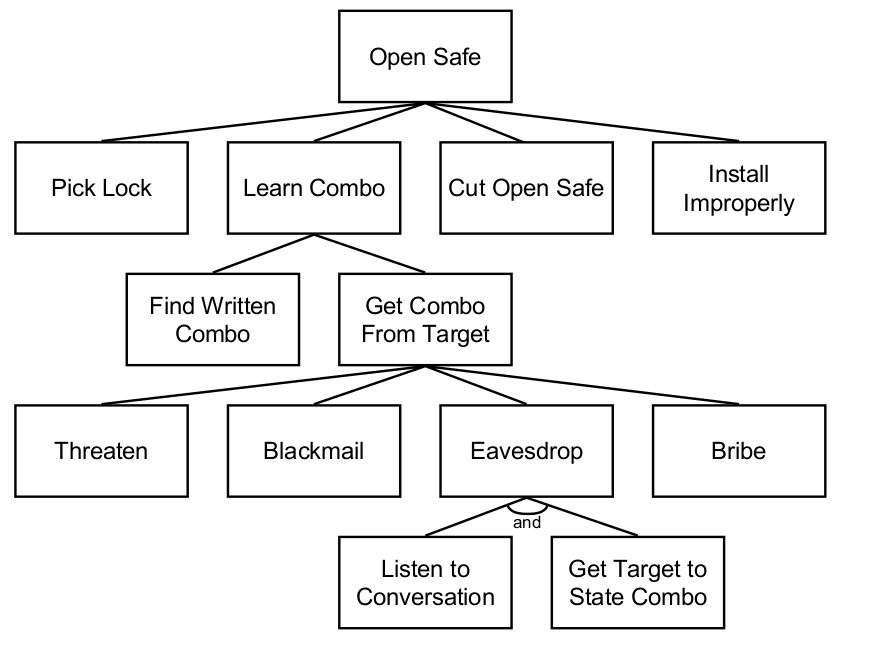
\includegraphics[scale=0.3]{img/tree.png}
\captionof{figure}{Exemple d'une attack tree}
\end{center}
\paragraph{}
Avec l'attack tree on peut représenter les attaques et les contre-mesures sachant que le noeud racine représente le but de l'attaque et les feuilles  représentent les différentes façons pour atteindre cet objectif, et aussi on peut associer à chaque noeud une varibale boolean(or,and) où une variable qui exprime le coût d'une attaque...etc.

\section{MulVal :}
En 2005 Ou et al. présentent MulVAL\cite{ref1} comme un framework open source qui permet de générer les graphes d'attaques pour analyser la sécurité des réseaux informatique. MulVal utilise Datalog comme un langage de modélisation et Prolog comme un moteur de raisonnement. Le temps d'exécution de \textit{MulVal scanner} est 236 secondes et \textit{MulVal engine} est capable de traiter un exemple de 2 000 machines en 16 secondes. La figure ci-dessous représente l'architecture de framework:
\begin{center}
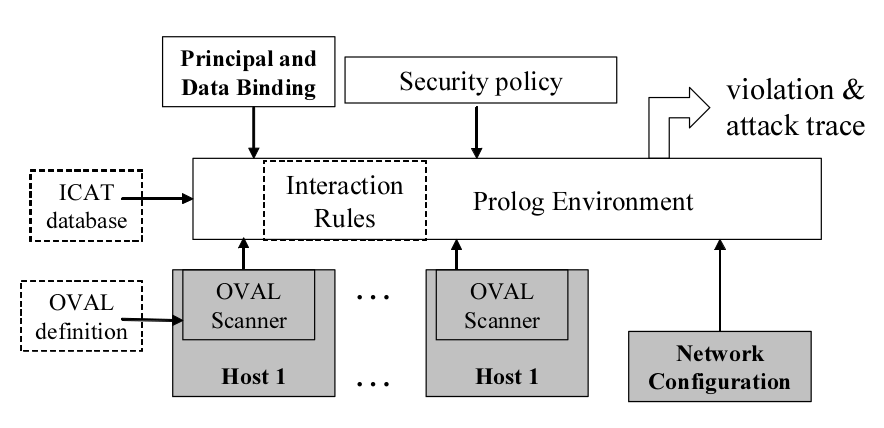
\includegraphics[scale=0.3]{img/MulVal.png}
\captionof{figure}{Architecture de MulVal framwork}
\end{center}

Ce framework possède deux logiciels. D'une part \textit{MulVal scanner} , qui permet d'analyser les configurations des machines et aussi déterminer les vulnérabilités qui existent et d'autre 	par \textit{MulVal engine} qui raisonne sur la configuration.
\paragraph{}
En 2006, Ou et al. proposent une évolution de MulVal nommée \textit{logical attack graph}\cite{ref6}. Ils ont démontré comment utiliser les traces d'attaques de MulVAl pour générer un \textit{logical attack graph} en temps quadratique.


\section{TVA :}
En 2005 . Sushil Jajodia et al\cite{ref2}.  présentent \textit{Topological Vulnerability Analysis (TVA)} comme un framework de génération des graphes d'attaques. La figure ci-dessous représente l'approche de TVA:
\begin{center}
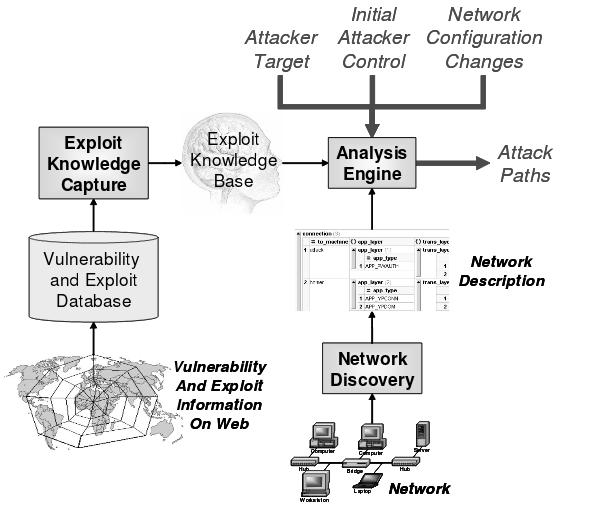
\includegraphics[scale=0.4]{img/TVA.png}
\captionof{figure}{Architecture de TVA}
\end{center}
\newpage
Ce framework possède trois composants : \textit{(1) une base de connaissances} regroupe l'ensemble de vulnérabilités et les règles de l'éxploitation, \textit{(2) la description de réseaux}, et \textit{(3) une spécification de scénario d'attaque}. Le moteur d'analyse TVA fusionne ces trois composantes et découvre  les chemins d'attaques. 

\section{NetSPA :}
En 2002. le Lincoln Laboratory du MIT démarre le projet \textit{Network Security Planning Architecture (NetSpa)}\cite{ref5} qui permet de générer automatiquement les graphes d'attaques à partir des actions modélisée avec REM un simple langage de description d'attaque . L'outil NetSpa est réalisé en C++ et dans sa première version, est capable de générer un graphe d'attaque à partir 17 machines en 1.5 minutes. La figure ci-dessous représente l'architecture NetSPA :
\begin{center}
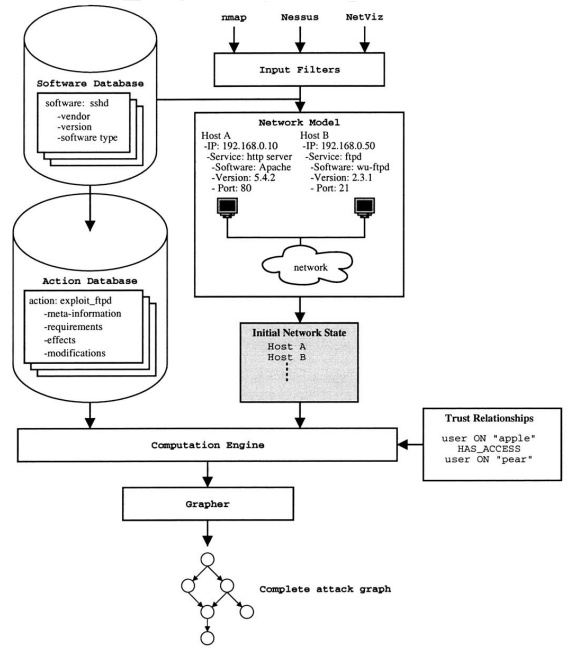
\includegraphics[scale=0.4]{img/NetSPA.png}
\captionof{figure}{Architecture de NetSPA}
\end{center}
\paragraph{}
En 2006, une nouvelle version de NetSPA est présentée\cite{ref3}, basée sur \textit{predictive graphs} qui sont des graphes d'attaques simplifiés. cette version est capable 	d'analyser des réseaux ayant jusqu'à 50 000 machines en moins de 4 minutes.
\newpage
\bibliography{mabiblio}
\bibliographystyle{plain}
\end{document}